%=====================================================================
%  Class 1 — Climate Impacts
%  FEA/USP — Climate Course, 2026
%
%  Built on the three papers in ../papers/:
%    [JEL]   Dell, Jones & Olken (2014), JEL 52(3) — the literature review
%    [DJO]   Dell, Jones & Olken (2012), AEJ: Macro 4(3) — application 1
%    [JMOvD] Jones, Moscona, Olken & von Dessauer (2026), NBER w34671 — application 2
%
%  Build:  python figures_src/build_all.py
%          pdflatex main.tex && pdflatex main.tex      (twice, for navigation)
%
%  Placeholders are [[like this]], never <like this> — beamer eats <...>.
%=====================================================================
\documentclass[aspectratio=169,10pt]{beamer}

\usepackage[english]{babel}
\usepackage{climatetheme}

\graphicspath{{figures/}}
\classfooter{Class 1 — Climate Impacts}

\title{Climate Course}
\subtitle{Climate Impacts}
\author{Nara Morais (FEA/USP)}
\institute{FEA/USP}
\date{2026}

% Compact table helpers: significance stars, standard errors, ragged p-columns.
\newcommand{\stars}[1]{\textsuperscript{#1}}
\newcommand{\se}[1]{{\scriptsize (#1)}}
\newcolumntype{L}[1]{>{\raggedright\arraybackslash}p{#1}}

% Diagram conventions, mirrored from class_empirics/main.tex so the two decks
% read the same way: right-angled grey connectors, and a three-level reading
% ramp inside every box — a mono uppercase eyebrow saying what the box answers,
% a bold name, and a muted sublabel carrying the detail. Keep the two in sync.
\usetikzlibrary{positioning,calc}

% Progressive reveal INSIDE a tikzpicture. Using \only would change the bounding
% box between overlays and make the whole diagram jump; this draws every element
% on every slide and simply sets opacity 0 until its turn, so nothing moves.
%   \node[visible on=<2->] ... ;
\tikzset{
  invisible/.style={opacity=0},
  visible on/.style={alt={#1{}{invisible}}},
  alt/.code args={<#1>#2#3}{\alt<#1>{\pgfkeysalso{#2}}{\pgfkeysalso{#3}}},
}

\newcommand{\dtag}[2]{{\ttfamily\scriptsize\color{#1}#2}}
\newcommand{\dsub}[1]{{\scriptsize\color{climgrey}#1}}

%=====================================================================
\begin{document}

\titleframe{Climate Impacts}{Estimating the economic effects of climate}
           {Identification, measurement, and two applications}

% ---- ROADMAP ----------------------------------------------------------
\begin{frame}{Outline}
  \vfill
  \begin{block}{Dell, Jones \& Olken (2014), \emph{Journal of Economic Literature}}
    \small How the effect of climate on an economic outcome can be identified at
    all, and what has to be decided before any regression can be run.
  \end{block}
  \vspace{2pt}
  \begin{block}{Dell, Jones \& Olken (2012), \emph{AEJ: Macroeconomics}}
    \small An application of that design, organised around a single testable
    question: does temperature affect the level of output or its growth rate?
  \end{block}
  \vspace{2pt}
  \begin{block}{Jones, Moscona, Olken \& von Dessauer (2026)}
    \small A recent paper arguing that the most common specification for
    nonlinear temperature effects is systematically biased, and proposing a
    correction.
  \end{block}
  \vfill
\end{frame}

% =====================================================================
\partframe{Part I}{What do we learn from the weather?}
% =====================================================================
\section{Part I — What do we learn from the weather?}

% ---------------------------------------------------------------------
\begin{frame}{Climate and weather}
  \[
    y \;=\; f(C,\; X)
  \]
  \begin{itemize}
    \item $y$ is an economic outcome: income, mortality, agricultural yields,
          conflict.
    \item $C$ denotes the \textbf{climate}, understood as the full probability
          distribution from which daily weather is drawn.
    \item $X$ collects everything else that determines the outcome: institutions,
          technology, the capital stock, policy.
  \end{itemize}
  \vspace{4pt}
  \begin{block}{Climate is a distribution; weather is a realisation of it}
    \small Rio de Janeiro's climate is what determines how you dress in general;
    the rain on a particular Tuesday is weather. The distinction matters because a
    regression of $y$ on observed weather estimates the effect of a realisation,
    whereas climate change is a change in the underlying distribution. Recovering
    the second from the first is the central problem of this literature.
  \end{block}
  \src{Dell, Jones \& Olken (2014), \emph{JEL}, Section 1}
\end{frame}

% ---------------------------------------------------------------------
% The fork in the literature, as one picture. Same drawing rules as Class 2:
% right-angled connectors in grey (an arrow is structure, not emphasis), and the
% accent spent on exactly one element. The two designs are deliberately drawn
% identically — same border, same fill, same tag colour — because they are peers
% and neither of them wins. The only accented box is the trade-off at the bottom,
% which is the thing the next frames actually argue about.
\begin{frame}{How can we measure it?}
  \vspace{-10pt}
  \begin{center}
  \begin{tikzpicture}[
      font=\small,
      card/.style   ={rounded corners=3pt, inner sep=4pt, align=center,
                      text=climdeep, font=\footnotesize},
      plain/.style  ={card, fill=white,        draw=climdeep!40,  line width=0.6pt},
      focal/.style  ={card, fill=climorange!7, draw=climorange!85, line width=0.7pt},
      ledger/.style ={anchor=north, inner sep=2pt, text=climdeep, font=\scriptsize},
      ar/.style     ={->, draw=climgrey, line width=0.7pt, rounded corners=3pt},
      link/.style   ={draw=climgrey, line width=0.7pt, rounded corners=3pt}]

    % --- the object of interest, and the reason it is hard --------------------
    \node[plain, text width=10.6cm] (root)
      {\dtag{climteal}{WHAT WE WANT}\\[2pt]
       $y = f(C,X)$\\[2pt]
       \dsub{the response of $y$ to the climate $C$ --- which varies across
             places, and so does everything in $X$}};

    % The stub below the root is where the literature forks. Both branches leave
    % from the same point and are the same length, so the picture cannot be read
    % as putting one design before the other.
    \coordinate (fork) at ([yshift=-0.35cm]root.south);
    \draw[link, visible on=<2->] (root.south) -- (fork);

    \node[plain, text width=6.3cm, anchor=north, visible on=<2->]
      (xs) at ([xshift=-3.5cm, yshift=-0.8cm]root.south)
      {\dtag{climteal}{COMPARES PLACES}\\[2pt]
       \textbf{The cross-section}\\[1pt]
       \dsub{different places with different climates,\\ at one point in time}};

    \node[plain, text width=6.3cm, anchor=north, visible on=<3->]
      (pn) at ([xshift=3.5cm, yshift=-0.8cm]root.south)
      {\dtag{climteal}{COMPARES YEARS}\\[2pt]
       \textbf{The panel}\\[1pt]
       \dsub{one place compared with itself,\\ year after year}};

    \draw[ar, visible on=<2->] (fork) -| (xs.north);
    \draw[ar, visible on=<3->] (fork) -| (pn.north);

    % --- what each design holds fixed, assumes, and therefore recovers --------
    % The leading \strut in the label cells is load-bearing, not decoration.
    % \dtag opens with \color, and a p-column whose first item is a colour
    % whatsit rather than a box has its height computed as zero, which drops
    % the label half a line below the text it labels. The strut gives the cell
    % a real first box. Remove it and the two columns stop lining up.
    \node[ledger, visible on=<2->] (xsl) at ([yshift=-0.18cm]xs.south)
      {\begin{tabular}{@{}L{1.75cm}@{\hspace{4pt}}L{4.35cm}@{}}
         \strut\dtag{climgrey}{HOLDS FIXED} & nothing. $X$ has to enter as a control. \\[2pt]
         \strut\dtag{climgrey}{ASSUMES}     & no omitted term correlated with $C$; and
                                              that $C$ did not itself shape $X$. \\[2pt]
         \strut\dtag{climgrey}{IDENTIFIES}  & a long-run response, with adaptation
                                              already in it. \\
       \end{tabular}};

    \node[ledger, visible on=<3->] (pnl) at ([yshift=-0.18cm]pn.south)
      {\begin{tabular}{@{}L{1.75cm}@{\hspace{4pt}}L{4.35cm}@{}}
         \strut\dtag{climgrey}{HOLDS FIXED} & everything time-invariant about a place,
                                              and every common shock. \\[2pt]
         \strut\dtag{climgrey}{ASSUMES}     & weather deviations are as good as random
                                              given those fixed effects. \\[2pt]
         \strut\dtag{climgrey}{IDENTIFIES}  & a short-run response, before adaptation
                                              has happened. \\
       \end{tabular}};

    % --- the trade-off the two designs are stuck with ------------------------
    \node[focal, text width=13.4cm, align=left, anchor=north, visible on=<4->]
      (band) at ([yshift=-0.4cm]$(xsl.south)!0.5!(pnl.south)$)
      {\dtag{climorange!85}{THE TRADE-OFF}\quad The cross-section has the right
       variation but the wrong identification; the panel has the right
       identification but arguably the wrong variation. The next frames take
       each one in turn.};

    \draw[ar, visible on=<4->] (xsl.south) -- (xsl.south |- band.north);
    \draw[ar, visible on=<4->] (pnl.south) -- (pnl.south |- band.north);

  \end{tikzpicture}
  \end{center}
  \vspace{-2pt}
  \src{Dell, Jones \& Olken (2014), \emph{JEL}, Sections 2.1--2.2}
\end{frame}

% ---------------------------------------------------------------------
\begin{frame}{The cross-sectional approach}
  \[
    y_i \;=\; \alpha \;+\; \beta\, C_i \;+\; \gamma\, X_i \;+\; \varepsilon_i
  \]
  \begin{itemize}
    \item The underlying correlation is large and well documented: across countries
          in 2000, a climate $1\,^\circ$C warmer is associated with income per capita
          roughly $8.5\%$ lower.
    \item What could go wrong?
      \begin{itemize}
        \item \textbf{Omitted variables.} Countries with hot climates also differ in
              colonial history, disease environment and institutional quality. If
              those differences enter $\varepsilon_i$, then
              $\mathrm{Cov}(C_i, \varepsilon_i) \neq 0$ and $\hat\beta$ is
              inconsistent.
        \item \textbf{Over-controlling.} Suppose instead that $X = X(C)$, so that
              climate itself shaped those institutions. Conditioning on $X$ then
              removes part of the effect we are trying to measure.
      \end{itemize}
  \end{itemize}
  \src{Dell, Jones \& Olken (2014), \emph{JEL}, Section 2.1}
\end{frame}

% ---------------------------------------------------------------------
% The paper's own Figure 1 rather than a rebuild: the scatter needs PWT/WDI
% income data, which we do not have offline. Cropped out of the source PDF by
% figures_src/crop_djo2012_fig1.tex, so it stays vector.
\begin{frame}{The cross-sectional correlation}
  \begin{columns}[T]
    \begin{column}{0.62\textwidth}
      \vspace{-4pt}
      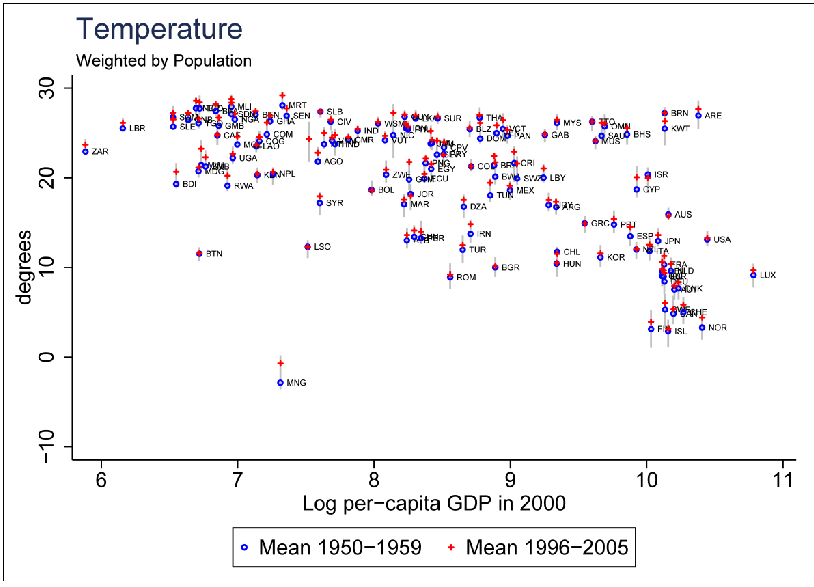
\includegraphics[width=\linewidth]{fig_djo2012_crosssection}
    \end{column}
    \begin{column}{0.35\textwidth}
      \small
      \begin{itemize}
        \item One point per country: population-weighted mean temperature against
              log GDP per capita in 2000.
        \item Circles are the 1950--1959 mean, crosses the 1996--2005 mean, the grey
              line the range of annual values in between.
        \item Mauritania at $28.4\,^\circ$C, Mongolia at $1.77\,^\circ$C; the slope
              is $-0.085$ log points per degree.
        \item The grey lines are short next to the spread across countries. That gap
              is what the panel design has to live on.
      \end{itemize}
    \end{column}
  \end{columns}
  \src{Dell, Jones \& Olken (2012), \emph{AEJ: Macro}, Figure 1 (temperature panel)}
\end{frame}

% ---------------------------------------------------------------------
\begin{frame}{The panel approach}
  \[
    y_{it} \;=\; \beta\, C_{it} \;+\; \mu_i \;+\; \theta_{rt} \;+\; \varepsilon_{it}
  \]
  \begin{itemize}
    \item The country fixed effects $\mu_i$ absorb all time-invariant determinants of
          the outcome, including institutions, geography, colonial history and the
          average climate itself.
    \item The region-by-year fixed effects $\theta_{rt}$ absorb shocks common to a
          group of countries in a given year, such as global commodity cycles.
    \item $\beta$ is therefore identified from year-to-year deviations of a country
          from its own long-run average, measured relative to other countries in the
          same region and year.
  \end{itemize}
  \vspace{4pt}
  \begin{block}{Identifying assumption}
    \small Conditional on $\mu_i$ and $\theta_{rt}$, the weather realisation
    $C_{it}$ is uncorrelated with $\varepsilon_{it}$. This assumption is unusually
    plausible by the standards of applied macroeconomics: a country's policies and
    economic conditions do not determine its own annual weather deviations.
  \end{block}
  \src{Dell, Jones \& Olken (2014), \emph{JEL}, Section 2.2}
\end{frame}

% ---------------------------------------------------------------------
\begin{frame}{Sources of weather data}
  \begin{center}
    \small
    \begin{tabular}{@{}L{0.22\textwidth}L{0.58\textwidth}@{}}
      \toprule
      \textbf{Type} & \textbf{Examples} \\
      \midrule
      Ground stations & GHCN-Daily \\[3pt]
      Interpolated grids & CRU, UDEL ($0.5^\circ\times0.5^\circ$), PRISM \\[3pt]
      Satellite & UAH, RSS ($2.5^\circ$), available from 1979 \\[3pt]
      Reanalysis & NCEP, ERA5-Land ($0.1^\circ$, hourly) \\
      \bottomrule
    \end{tabular}
  \end{center}
  \vspace{2pt}
  \begin{itemize}
    \small
    \item None of these is ``the temperature''. Stations observe, grids interpolate
          between stations, satellites measure the atmosphere rather than the
          surface, and reanalysis is a weather model fitted to whatever observations
          exist.
    \item Coverage is not stable over time either: the number of reporting GHCN
          stations falls sharply around 1990 with the dissolution of the USSR, which
          is a break in the data rather than in the climate.
    \item Papers routinely report results for more than one product, and sensitivity
          to that choice is a warning sign.
  \end{itemize}
  \src{Dell, Jones \& Olken (2014), \emph{JEL}, Section 2.3 and Figure 1}
\end{frame}

% ---------------------------------------------------------------------
\begin{frame}{How to model climate variables?}
  Between a gridded weather product and the regressor $C_{it}$ there are three
  decisions, none of which is innocuous.
  \vspace{4pt}
  \begin{enumerate}
    \item \textbf{Which product.} Stations, interpolated grids, satellite or
          reanalysis. Products disagree with one another, and they disagree more
          about rainfall than about temperature.
    \item \textbf{How to aggregate space.} A grid cell is not a country. The cells
          have to be averaged into the unit of analysis, and the weights used ---
          area or population --- are a substantive choice rather than a technical
          one.
    \item \textbf{Which functional form, and over what period.} Whether temperature
          enters linearly, in bins, as an anomaly or as degree-days, and whether it
          is averaged before or after that transformation.
  \end{enumerate}
  \src{Dell, Jones \& Olken (2014), \emph{JEL}, Sections 2.3--2.4}
\end{frame}

% ---------------------------------------------------------------------
\begin{frame}{Aggregation and measurement error}
  \begin{block}{Aggregating grid cells to a country}
    \small Area weights treat uninhabited territory and dense urban areas equally;
    population weights instead weight by exposure. For the United States in 2000 the
    two give
    \[
      \bar{T}^{\text{area}} = 8.3\,^\circ\mathrm{C}
      \qquad\text{and}\qquad
      \bar{T}^{\text{pop}} = 13.1\,^\circ\mathrm{C}
    \]
    a difference of $4.8\,^\circ$C, larger than a century of observed warming.
  \end{block}
  \begin{block}{Precipitation is measured less reliably than temperature}
    \small Temperature is spatially smooth; rainfall is not. The correlation of
    deviations across data products is $0.92$ for temperature but only $0.70$ for
    precipitation. A null result on rainfall may therefore reflect attenuation from
    measurement error rather than the absence of an effect.
  \end{block}
  \src{Dell, Jones \& Olken (2014), \emph{JEL}, Section 2.3}
\end{frame}

% ---------------------------------------------------------------------
\begin{frame}{Functional form}
  \small
  \begin{enumerate}
    \item \textbf{Levels}: $\beta\,T_{it}$. A single parameter, which imposes that the
          marginal effect of one degree is the same at $5\,^\circ$C and at
          $35\,^\circ$C.
    \item \textbf{Bins}: $\sum_k \beta_k\, T_{kit}$, where $T_{kit}$ counts days spent
          in temperature range $k$. This imposes no shape on the response and is the
          specification discussed in Part III.
    \item \textbf{Anomalies}: $(T_{it}-\bar T_i)/\sigma_i$. Comparable across places
          with very different climates, at the cost of a normalisation.
    \item \textbf{Degree-days}: $\int \max(0, T - \underline{T})\,dt$, motivated by
          crop biology. Schlenker and Roberts (2009) estimate thresholds of
          $29\,^\circ$C for corn, $30\,^\circ$C for soybeans and $32\,^\circ$C for
          cotton.
  \end{enumerate}
  \vspace{4pt}
  \begin{block}{Temporal aggregation}
    \small If temperature is averaged before being binned, the nonlinearity of
    interest is averaged away: a month with a mean of $24\,^\circ$C may contain a week
    above $32\,^\circ$C or none at all.
  \end{block}
  \src{Dell, Jones \& Olken (2014), \emph{JEL}, Section 2.4}
\end{frame}

% =====================================================================
\partframe{Part II}{Temperature shocks and economic growth}
% =====================================================================
\section{Part II — Levels or growth? (DJO 2012)}

% ---------------------------------------------------------------------
\begin{frame}{Dell, Jones \& Olken (2012)}
  \begin{block}{Research question}
    \small Does a temperature shock reduce the \emph{level} of output in the year in
    which it occurs, or the \emph{rate of growth}, so that output never returns to
    its previous path? The two are difficult to tell apart in a single year and
    imply damages that differ by orders of magnitude over a century.
  \end{block}
  \vspace{2pt}
  \small
  \begin{itemize}
    \item \textbf{Setting.} All countries with population above one million,
          1950--2003, annual; $n = 4{,}924$ country-years.
    \item \textbf{Data.} Temperature and precipitation from Matsuura and Willmott
          ($0.5^\circ$ grid, population-weighted to the country); GDP per capita from
          the World Development Indicators, with the Penn World Table as a
          robustness check.
    \item \textbf{Design.} A distributed lag in temperature with country fixed
          effects, region-by-year and poor-by-year fixed effects, and standard errors
          clustered by country and by region-year.
    \item \textbf{Headline result.} An increase of $1\,^\circ$C reduces growth in
          poor countries by about $1.4$ percentage points, and the loss is not
          recovered in subsequent years. No effect is detected in rich countries.
  \end{itemize}
  \src{Dell, Jones \& Olken (2012), \emph{AEJ: Macro}}
\end{frame}

% ---------------------------------------------------------------------
\begin{frame}{Levels versus growth}
  \begin{columns}[T]
    \begin{column}{0.47\textwidth}
      \begin{block}{A level effect}
        \small A hot year reduces output in that year. In the following year, with
        normal weather, output returns to its previous trend. The growth path is
        unchanged.
      \end{block}
    \end{column}
    \begin{column}{0.47\textwidth}
      \begin{block}{A growth effect}
        \small A hot year reduces the rate at which capital, productivity or
        institutional capacity accumulate. Output does not return to its previous
        path, which is permanently lower.
      \end{block}
    \end{column}
  \end{columns}
  \vspace{6pt}
  \begin{itemize}
    \item Integrated assessment models almost always make this choice by assumption,
          writing damages as $D(T)\,A_t F(K,L)$: temperature scales the level of
          output, and growth is left untouched.
    \item The alternative is $\log A_t = \log A_{t-1} + g(T)$, in which a hot year
          lowers the whole subsequent path. Here the choice between the two is
          treated as a hypothesis to be tested rather than a modelling convention.
    \item Over a century the difference is not a technicality: it is the difference
          between damages of a few per cent of output and damages several times
          larger.
  \end{itemize}
  \src{Dell, Jones \& Olken (2012), \emph{AEJ: Macro}, Section I}
\end{frame}

% ---------------------------------------------------------------------
\begin{frame}{A model in which both channels are present}
  Let temperature affect both the level of productivity and its rate of change:
  \[
    Y_{it} \;=\; e^{\beta T_{it}}\, A_{it}\, L_{it},
    \qquad
    \frac{\Delta A_{it}}{A_{it}} \;=\; g_i \;+\; \gamma\, T_{it}
  \]
  Taking logarithms and first differences gives growth in output per capita as
  \[
    \boxed{\;g_{it} \;=\; g_i \;+\; (\beta + \gamma)\,T_{it} \;-\; \beta\,T_{it-1}\;}
  \]
  \begin{itemize}
    \item The level parameter $\beta$ enters contemporaneously with coefficient
          $+\beta$ and enters again in the following period with coefficient
          $-\beta$: its contribution to the sum of the coefficients is zero.
    \item The growth parameter $\gamma$ enters once and is not reversed.
    \item The sum of the distributed-lag coefficients therefore distinguishes the two
          channels, and this is what the empirical work exploits.
  \end{itemize}
  \src{Dell, Jones \& Olken (2012), equations (1)--(3)}
\end{frame}

% ---------------------------------------------------------------------
\begin{frame}{The estimating equation}
  \[
    g_{it} \;=\; \mu_i \;+\; \theta_{rt}
    \;+\; \sum_{j=0}^{L} \rho_j\, T_{it-j} \;+\; \varepsilon_{it}
  \]
  \small
  \begin{itemize}
    \item $\mu_i$ denotes country fixed effects, so that identification comes from a
          country's own deviations from its mean.
    \item $\theta_{rt}$ denotes region-by-year and poor-by-year fixed effects. A poor
          country is therefore compared with other poor countries in the same year
          rather than with the OECD.
    \item Standard errors are clustered in two dimensions, by country and by
          region-year, following Cameron, Gelbach and Miller: weather is serially
          correlated within a country and spatially correlated across neighbours.
    \item First differencing is preferred to a levels specification with a lagged
          dependent variable because of Nickell bias; Bond, Leblebicio\u{g}lu and
          Schiantarelli (2010) show that with $T$ large the first-differenced
          estimator is preferable in growth regressions.
    \item ``Poor'' is defined as below-median PPP GDP per capita in the country's
          first year in the sample. The classification is fixed, so it cannot itself
          be an outcome of temperature.
  \end{itemize}
  \src{Dell, Jones \& Olken (2012), equation (4)}
\end{frame}

% ---------------------------------------------------------------------
\begin{frame}{Hypotheses}
  \vfill
  \begin{block}{Without lags ($L=0$): \quad $H_0: \ \rho_0 = 0$}
    \small Temperature has no contemporaneous association with growth.
  \end{block}
  \vspace{2pt}
  \begin{block}{With lags ($L>0$): \quad $H_0^{1}: \ \rho_0 = 0$}
    \small Temperature has no immediate effect once dynamics are allowed for.
  \end{block}
  \vspace{2pt}
  \begin{block}{With lags ($L>0$): \quad $H_0^{2}: \ \sum_{j=0}^{L}\rho_j = 0$}
    \small This is the hypothesis of interest. Under a pure level effect the lagged
    terms offset the contemporaneous term and the sum is zero. Rejecting $H_0^2$
    indicates that the shock is not recovered, which is the signature of a growth
    effect.
  \end{block}
  \vfill
  \centering\small
  $H_0^2$ is a restriction on a linear combination of coefficients rather than on a
  single coefficient, which is why the covariance structure of the errors matters.
\end{frame}

% ---------------------------------------------------------------------
\begin{frame}{Main results}
  \centering
  \small Dependent variable: growth in GDP per capita, 1950--2003, $n = 4{,}924$.
  \vspace{4pt}

  \footnotesize
  \begin{tabular}{@{}lc@{}}
    \toprule
    \multicolumn{2}{@{}l}{\textbf{Panel A. Effect of $+1\,^\circ$C on annual growth (pp)}} \\
    \midrule
    Temperature, all countries pooled       & $-0.325$ \se{0.285} \\
    Temperature, rich countries             & $\phantom{-}0.261$ \se{0.312} \\
    Temperature $\times$ Poor               & $-1.655$\stars{***} \se{0.485} \\
    \textbf{Implied effect in poor countries} & $\mathbf{-1.394}$\stars{***} \se{0.408} \\
    \quad with precipitation controls       & $-1.347$\stars{***} \se{0.408} \\
    \midrule
    \multicolumn{2}{@{}l}{\textbf{Panel B. Alternative interactions}} \\
    \midrule
    \quad including Temperature $\times$ Hot          & $-1.473$\stars{***} \\
    \quad including Temperature $\times$ Agricultural & $-1.245$\stars{***} \\
    \midrule
    Precipitation, poor countries (per 100 mm) & $\phantom{-}0.069$ \se{0.058} \\
    Precipitation, rich countries              & $-0.083$\stars{*} \se{0.050} \\
    \bottomrule
  \end{tabular}
  \vspace{3pt}
  \\ \scriptsize One standard deviation of the temperature shock is $0.50\,^\circ$C,
  implying a cost of about $0.69$ percentage points of growth. Panel B shows that
  interactions with ``hot'' or ``agricultural'' do not displace the interaction with
  income.
  \src{Dell, Jones \& Olken (2012), \emph{AEJ: Macro}, Table 2}
\end{frame}

% ---------------------------------------------------------------------
\begin{frame}{Cumulative effects of lagged temperature}
  \begin{columns}[T]
    \begin{column}{0.54\textwidth}
      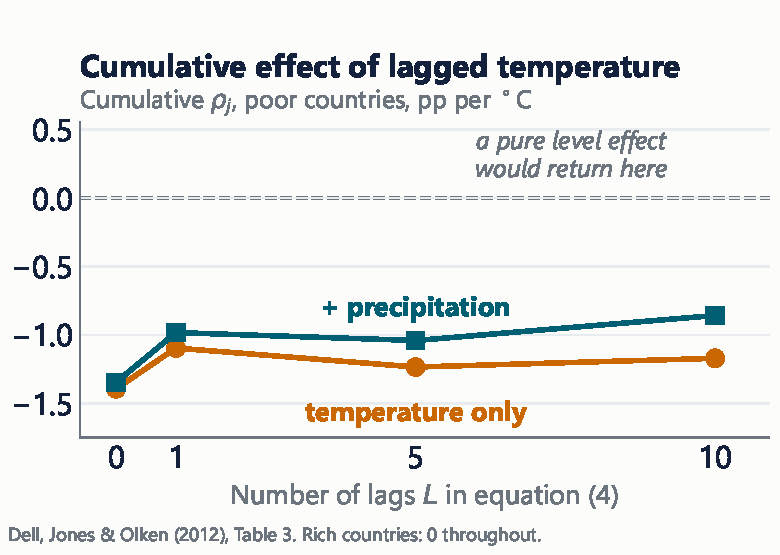
\includegraphics[width=\linewidth]{fig04_lagsums}
    \end{column}
    \begin{column}{0.42\textwidth}
      \small
      \begin{itemize}
        \item Under a pure level effect, $\sum_j \rho_j$ should approach zero as lags
              are added (dashed line).
        \item The estimated sums do not. At ten lags they remain at $-1.17$ without
              precipitation controls and $-0.86$ with them.
        \item For rich countries the sums are indistinguishable from zero at every
              lag length.
        \item $H_0^2$ is therefore rejected for poor countries: the effect is on
              growth, not only on levels.
      \end{itemize}
    \end{column}
  \end{columns}
  \vspace{2pt}
  \scriptsize
  On precision: with ten lags and two-way clustering the estimates are imprecise, and
  the ten-lag sum with precipitation controls is no longer significant at the $5\%$
  level. The evidence is the pattern across lag lengths, not any single column.
  \src{Dell, Jones \& Olken (2012), \emph{AEJ: Macro}, Table 3}
\end{frame}

% ---------------------------------------------------------------------
\begin{frame}{Robustness}
  \centering
  \small Immediate effect of $+1\,^\circ$C on growth in poor countries, percentage
  points.
  \vspace{4pt}

  \footnotesize
  \begin{tabular}{@{}lc@{}}
    \toprule
    \textbf{Specification} & \textbf{Estimate} \\
    \midrule
    Baseline, with precipitation controls & $-1.347$\stars{***} \\
    Including country-specific time trends & $-1.723$\stars{***} \\
    Balanced panel & $-1.377$\stars{***} \\
    Wider sample, including small countries & $-1.158$\stars{***} \\
    Penn World Table income in place of WDI & $-0.860$\stars{***} \\
    Area-weighted rather than population-weighted temperature & $-0.891$\stars{**} \\
    Sub-Saharan Africa only & $-1.881$\stars{***} \\
    Sub-Saharan Africa excluded & $-0.904$\stars{*} \\
    \bottomrule
  \end{tabular}
  \vspace{4pt}
  \\ \small The point estimate ranges between roughly $-0.9$ and $-1.9$ across
  specifications, while the sign and statistical significance are stable. The last two
  rows indicate that the result is not driven by Sub-Saharan Africa.
  \src{Dell, Jones \& Olken (2012), \emph{AEJ: Macro}, Table 4}
\end{frame}

% ---------------------------------------------------------------------
\begin{frame}{Sectoral decomposition}
  \begin{columns}[T]
    \begin{column}{0.52\textwidth}
      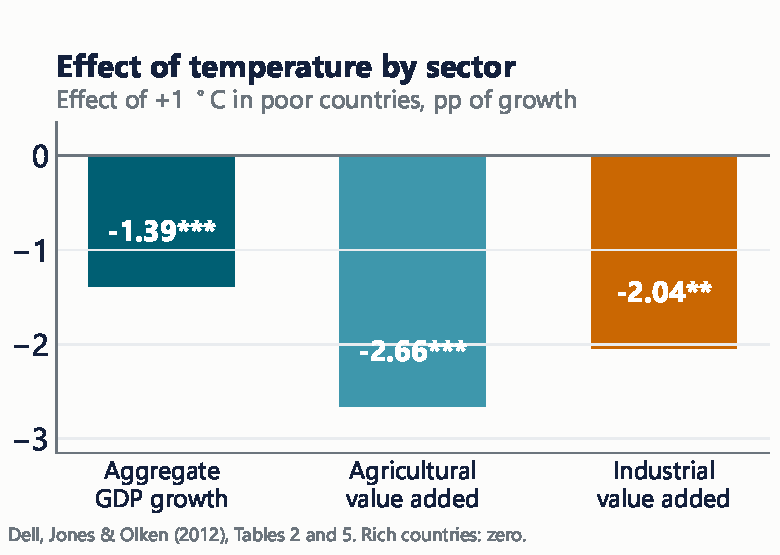
\includegraphics[width=\linewidth]{fig05_channels}
    \end{column}
    \begin{column}{0.44\textwidth}
      \small
      \begin{itemize}
        \item Agricultural value added responds most strongly, which is the expected
              result.
        \item Industrial value added falls by $2.04$ percentage points per
              $1\,^\circ$C, which is not readily explained by an agricultural
              mechanism.
        \item The estimated effect on investment is negative but not statistically
              significant.
        \item Precipitation has little measurable effect even in agriculture
              ($+0.18$ percentage points per 100 mm, not significant).
        \item The breadth of the response across sectors is part of what supports the
              growth interpretation.
      \end{itemize}
    \end{column}
  \end{columns}
  \src{Dell, Jones \& Olken (2012), \emph{AEJ: Macro}, Table 5}
\end{frame}

% ---------------------------------------------------------------------
\begin{frame}{Summary of Part II}
  \begin{enumerate}
    \item A model in which temperature affects both the level and the growth of
          productivity generates distinct predictions for the distributed-lag
          coefficients.
    \item The specification is a distributed lag with country and region-by-year fixed
          effects and two-way clustered standard errors.
    \item An increase of $1\,^\circ$C reduces growth in poor countries by about $1.4$
          percentage points. For rich countries no effect is detected.
    \item The sum of the lag coefficients does not return to zero, which is consistent
          with an effect on growth rather than on levels.
    \item The response appears in agriculture, in industry and in the probability of
          an irregular leadership transition.
    \item Medium-run estimates are no smaller, but the seven-year calibration shows
          that the relationship cannot be extrapolated over a century.
  \end{enumerate}
\end{frame}

% =====================================================================
\partframe{Part III}{With or without U? Binning bias}
% =====================================================================
\section{Part III — Binning bias (JMOvD 2026)}

% ---------------------------------------------------------------------
\begin{frame}{Jones, Moscona, Olken \& von Dessauer (2026)}
  \begin{block}{Research question}
    \small Binned panel regressions consistently produce a U-shaped response of
    economic outcomes to temperature, with both extremes appearing damaging. Is that
    shape a property of the economy, or is part of it produced by the specification
    itself?
  \end{block}
  \vspace{2pt}
  \small
  \begin{itemize}
    \item \textbf{Setting.} United States counties, with four outcomes taken from four
          established literatures: population (1970--2010), mortality above age 65
          (1970--2002), corn yields (1985--2006) and violent crime (1960--2009).
    \item \textbf{Data.} ERA5-Land reanalysis, $0.1^\circ$ and hourly from 1970,
          assigned to counties and counted into ten bins of $10\,^\circ$F.
    \item \textbf{Design.} The bias is derived analytically, confirmed in simulations
          in which the true effect of every bin is zero by construction, and then a
          correction is proposed and applied to the four literatures.
    \item \textbf{Headline result.} Of the four published patterns, one is reversed,
          one substantially weakened, one strengthened, and one unaffected.
  \end{itemize}
  \src{Jones, Moscona, Olken \& von Dessauer (2026), NBER Working Paper 34671}
\end{frame}

% ---------------------------------------------------------------------
\begin{frame}{The binned specification}
  \[
    Y_{it} \;=\; \alpha_i \;+\; \delta_t
    \;+\; \sum_k \beta_k\, T_{kit} \;+\; u_{it}
  \]
  \begin{itemize}
    \item $T_{kit}$ counts the days that unit $i$ spends in temperature bin $k$ during
          year $t$; a common choice is ten bins of $10\,^\circ$F, from below
          $10\,^\circ$F to above $90\,^\circ$F.
    \item The specification imposes no functional form, which is why it was described
          earlier as the appropriate way to estimate a nonlinear response.
    \item Estimates obtained this way are strikingly consistent across outcomes: a
          U-shape for mortality, crime and energy demand, and an inverted U for output
          and agricultural yields. Extreme temperatures appear damaging in both
          directions.
    \item These coefficients enter damage functions directly, and through them the
          social cost of carbon.
  \end{itemize}
  \vspace{2pt}
  \centering\color{climred}The argument of this paper is that part of the estimated
  U-shape is an artefact of warming itself.
  \src{Jones, Moscona, Olken \& von Dessauer (2026), equation (1)}
\end{frame}

% ---------------------------------------------------------------------
\begin{frame}{An illustration: Boston and Phoenix}
  \centering
  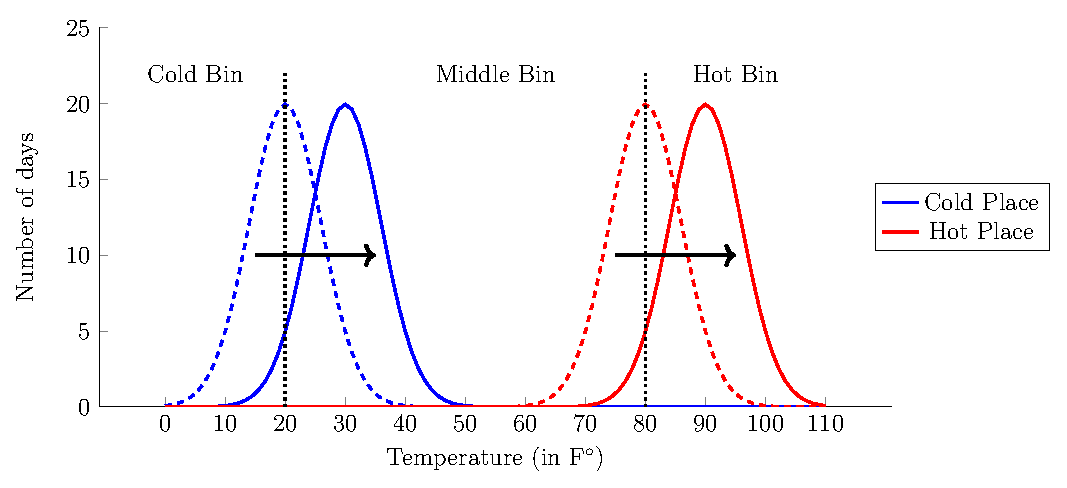
\includegraphics[width=0.50\linewidth]{fig_jmovd_uniformwarming}

  \vspace{1pt}
  {\small Warming of the same size moves both distributions equally, but only the hot
  place has days to push into the top bin, and only the cold place has cold days
  left to lose.}

  \vspace{5pt}
  {\small The same asymmetry in observed data: days per decade in the extreme bins,
  1970s against 2010s.}
  \vspace{2pt}

  \footnotesize
  \begin{tabular}{@{}lcccc@{}}
    \toprule
    & \multicolumn{2}{c}{\textbf{Days below $10\,^\circ$F}} & \multicolumn{2}{c}{\textbf{Days above $90\,^\circ$F}} \\
    \cmidrule(lr){2-3}\cmidrule(lr){4-5}
    & 1970s & 2010s & 1970s & 2010s \\
    \midrule
    Boston  & 20 & 10 & 0       & 0       \\
    Phoenix & 0  & 0  & 1{,}000 & 1{,}062 \\
    \bottomrule
  \end{tabular}

  \vspace{4pt}
  {\small The trend in an extreme bin is therefore a property of baseline climate,
  not of response to heat.}
  \src{Jones, Moscona, Olken \& von Dessauer (2026), Figure 1 and Table 1; ERA5-Land}
\end{frame}

% ---------------------------------------------------------------------
\begin{frame}{Why exposure to the extreme bins trends unevenly}
  \begin{columns}[T]
    \begin{column}{0.52\textwidth}
      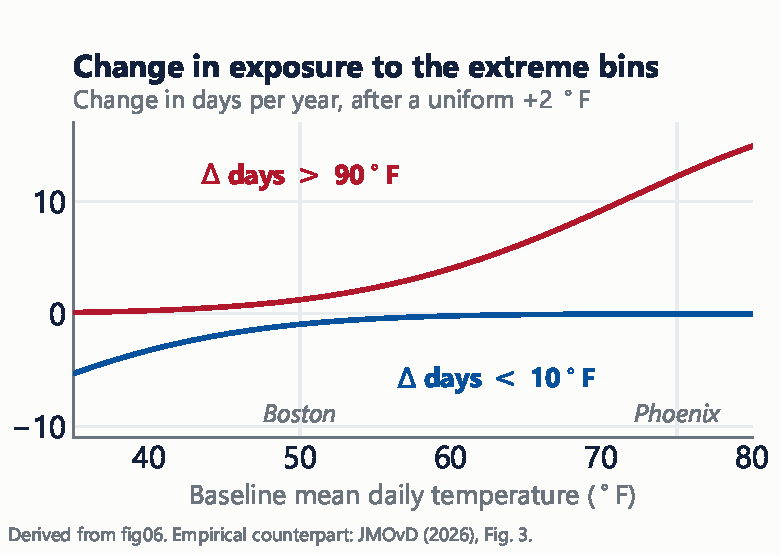
\includegraphics[width=\linewidth]{fig07_binshift}
    \end{column}
    \begin{column}{0.44\textwidth}
      \small
      If daily temperature is distributed $\mathcal{N}(\mu_i,\sigma^2)$ and warming
      shifts the mean by $\delta$, then to a first approximation
      \[
        \Delta\,\text{days}_{<10} \approx -365\,\phi\!\left(\tfrac{10-\mu_i}{\sigma}\right)\tfrac{\delta}{\sigma}
      \]
      \begin{itemize}
        \item Both changes are increasing in the baseline mean $\mu_i$: warmer places
              gain more hot days and lose fewer cold days.
        \item No economic behaviour is involved; this follows from the shape of the
              distribution.
        \item Across US counties both relationships are observed, positive and
              significant at $p \le 0.001$, while the moderate bins are flat.
      \end{itemize}
    \end{column}
  \end{columns}
  \src{Derived here; empirical counterpart in JMOvD (2026), Figure 3}
\end{frame}

% ---------------------------------------------------------------------
\begin{frame}{The source of the bias}
  \small
  Suppose the true model contains a place-specific trend that the researcher does not
  include:
  \[
    Y_{it} = \alpha_i + \delta_t + \sum_k \beta_k T_{kit}
    + \underbrace{\lambda_i t}_{\text{omitted}} + \varepsilon_{it}
  \]
  and let the bin counts themselves trend at place-specific rates:
  \[
    C_{it} = \mu_{C,i} + \varphi_{C,i}\,t + v_{C,it},
    \qquad
    H_{it} = \mu_{H,i} + \varphi_{H,i}\,t + v_{H,it}
  \]
  The researcher estimates the model without $\lambda_i t$, so that the error term is
  $u_{it} = \lambda_i t + \varepsilon_{it}$.
  \vspace{4pt}
  \begin{block}{Result 1}
    \small The bias in $\hat\beta_C$ and $\hat\beta_H$ is a function of the variances
    and covariances of $(\varphi_C, \varphi_H, \lambda)$ across places. This is
    omitted-variable bias in its standard form. What is specific to this setting is
    that the omitted variable is time itself, and its correlation with the regressor
    is guaranteed by the physical argument on the previous slide.
  \end{block}
  \src{Jones, Moscona, Olken \& von Dessauer (2026), Section 2, equations (2)--(8)}
\end{frame}

% ---------------------------------------------------------------------
\begin{frame}{Result 2: the shape of the bias}
  \small Let each trend be linear in the location's baseline temperature $T_{0,i}$:
  \[
    \varphi_{C,i} = a_C + b_C T_{0,i} + e_{C,i},\quad
    \varphi_{H,i} = a_H + b_H T_{0,i} + e_{H,i},\quad
    \lambda_i = a_Y + b_Y T_{0,i} + e_{Y,i}
  \]
  \vspace{-10pt}
  \centering
  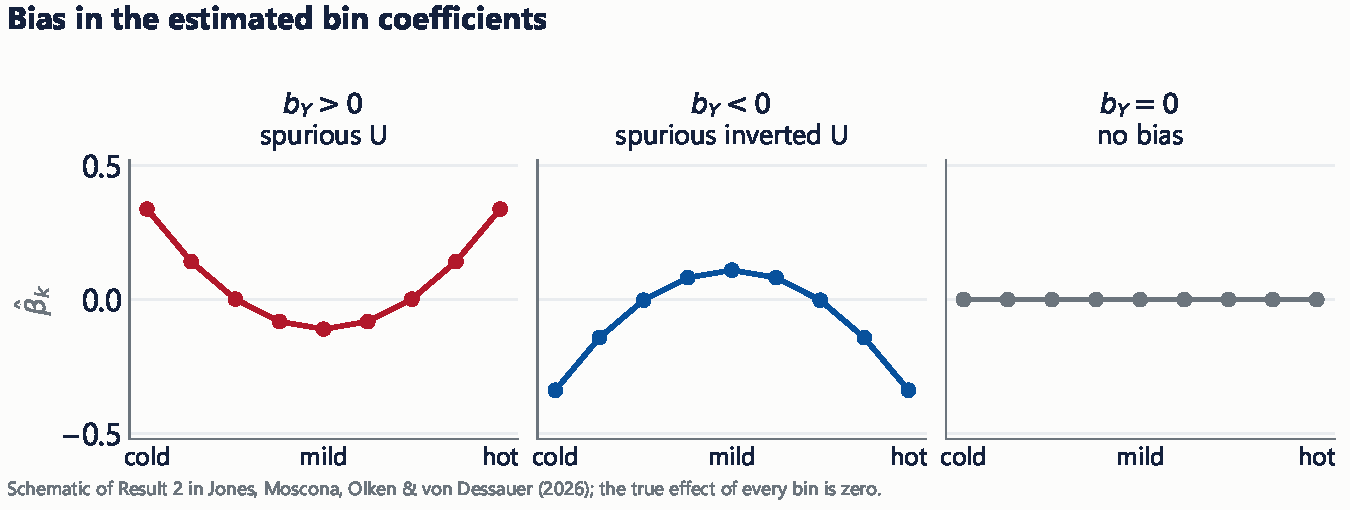
\includegraphics[width=0.88\linewidth]{fig08_taxonomy}

  \vspace{9pt}
  {\small The sign of $b_Y$ asks whether the outcome trends differently in places
  that were already hot.}
  \src{Jones, Moscona, Olken \& von Dessauer (2026), Result 2}
\end{frame}

% ---------------------------------------------------------------------
\begin{frame}{Four implications}
  \small
  \begin{enumerate}
    \item The bias is increasing in $b_Y$. Any process that causes hot places to trend
          differently --- migration to the Sun Belt, the diffusion of air conditioning,
          irrigation, divergent regional growth --- will generate it.
    \item The bias is decreasing in the noise in the trends. Idiosyncratic variation in
          local trends is protective, so systematic and precisely estimated trends are
          the more dangerous case.
    \item Longer panels make the problem worse. As $T$ increases, the deterministic
          component of the bin counts grows relative to the idiosyncratic year-to-year
          variation, so a larger share of the identifying variation is trend. Adding
          years of data does not attenuate the bias.
    \item Weak but precisely estimated trend relationships are the least favourable
          case, producing large and statistically significant coefficients with no
          underlying effect.
  \end{enumerate}
  \vspace{4pt}
  \begin{block}{}
    \small In simulations calibrated so that the true effect of every bin is zero, the
    top and bottom bins reject the null far more often than $5\%$ of the time, and the
    estimated response resembles those reported in the published literature.
  \end{block}
  \src{Jones, Moscona, Olken \& von Dessauer (2026), Sections 2 and 4}
\end{frame}

% ---------------------------------------------------------------------
\begin{frame}{Spurious evidence of adaptation}
  \begin{itemize}
    \item The conventional test for adaptation compares hot and cold counties and asks
          whether hot counties are less affected by hot days. A smaller estimated
          effect in hot counties is read as evidence that agents have adapted.
    \item In the simulation, where by construction no agent adapts because no bin has
          any effect, exactly this pattern emerges.
  \end{itemize}
  \vspace{4pt}
  \centering
  \footnotesize
  \begin{tabular}{@{}lcc@{}}
    \toprule
    \textbf{Simulated bias in} & \textbf{Hot counties} & \textbf{Cold counties} \\
    \midrule
    the cold bin (below $10\,^\circ$F) & $28.58$ & $0.72$ \\
    the hot bin (above $90\,^\circ$F)  & $1.60$  & $6.41$ \\
    \bottomrule
  \end{tabular}
  \vspace{4pt}
  \\ \small The asymmetry is not driven by steeper trends in these subsamples but by
  lower noise: cold counties have very stable counts of cold days, so the systematic
  component dominates.
  \src{Jones, Moscona, Olken \& von Dessauer (2026), Figure 6 and Table A.2}
\end{frame}

% ---------------------------------------------------------------------
\begin{frame}{A correction based on counterfactual exposure}
  \small
  For each place and year, construct the expected number of days in each bin under a
  counterfactual distribution $F_{ct}$ containing only the systematic trend:
  \[
    \bar T_{k,ct} \;=\; 365 \times \big(F_{ct}(\bar x) - F_{ct}(\underline{x})\big)
  \]
  and include it in the regression alongside the realised counts:
  \[
    Y_{ct} \;=\; \alpha_c + \delta_t
    + \sum_k \beta_k T_{kct}
    + \sum_k \gamma_k \bar T_{k,ct} + u_{ct}
  \]
  \begin{itemize}
    \item $\beta_k$ is then identified from the unexpected component of exposure,
          which is weather in the sense used at the start of the class, rather than
          from the trend.
    \item The logic is that of a control function (Wooldridge 2015), and it is the same
          idea as in Borusyak and Hull (2023) on non-random exposure to exogenous
          shocks: the shock is recentred on its expectation.
  \end{itemize}
  \src{Jones, Moscona, Olken \& von Dessauer (2026), equations (20)--(21)}
\end{frame}

% ---------------------------------------------------------------------
\begin{frame}{Constructing the counterfactual distribution}
  \small
  \begin{enumerate}
    \item For each county $c$ and calendar month $m$, regress daily mean temperature
          on a linear time trend:
          $\bar x_{cmt} = \mu_{cm} + \varphi_{cm} t + \varepsilon_{cmt}$.
    \item Shrink the estimated trends towards the national mean using an empirical
          Bayes adjustment, so that noisily estimated county-months do not drive the
          counterfactual.
    \item Remove the trend from every daily observation:
          $x^{\,\text{detrended}}_{cdmt} = x_{cdmt} - \hat\varphi_{cm}\,t$.
    \item Pool the de-trended observations within a county-month. For January in a
          single county this gives approximately $31 \times 50 = 1{,}550$ draws, which
          serve as an estimate of the shape of the local distribution.
    \item Project the distribution forward using $\hat\varphi_{cm}$ to obtain
          $F_{cmt}$, aggregate months to a county-year distribution $F_{ct}$, and
          compute the expected bin counts from equation (20).
  \end{enumerate}
  \vspace{4pt}
  The procedure uses only the temperature data, so it can be reproduced in any
  application; the authors distribute it as the Stata package \texttt{cftemp}.
  \src{Jones, Moscona, Olken \& von Dessauer (2026), Section 5.1, equations (22)--(23)}
\end{frame}

% ---------------------------------------------------------------------
\begin{frame}{Alternative strategies}
  
  \centering
  \footnotesize
  \begin{tabular}{@{}L{0.38\textwidth}cL{0.42\textwidth}@{}}
    \toprule
    \textbf{Strategy} & \textbf{Corrects the bias?} & \textbf{Assessment} \\
    \midrule
    State-by-year fixed effects & \color{climred}No
      & The top and bottom bins still reject falsely at $26\%$ and $14\%$. The
        apparent improvement comes from added noise rather than reduced bias. \\[3pt]
    Five lags of $Y$ and of $X$ & \color{climred}No
      & False rejection rates exceed $90\%$. Lags absorb common dynamics but not
        place-specific ones. \\[3pt]
    Place-specific linear trends & \color{climorange}Partly
      & Adequate when the outcome trend is genuinely linear; fails under quadratic or
        cubic trends, and requires more than 3{,}000 additional parameters. \\[3pt]
    County-by-five-year-period fixed effects & \color{climorange}Partly
      & Removes the bias in simulation, including with nonlinear trends, but requires
        annual data and is therefore unavailable for decadal outcomes or long
        differences. \\[3pt]
    Counterfactual bin counts, eq. (21) & \color{climteal}Yes
      & Estimates are centred at zero when there is no effect and recover the true
        effect when there is one. The correction operates on the right-hand side,
        which is why it generalises across outcomes. \\
    \bottomrule
  \end{tabular}
  \src{Jones, Moscona, Olken \& von Dessauer (2026), Sections 5.1--5.2}
\end{frame}

% ---------------------------------------------------------------------
\begin{frame}{Applications}
  \centering
  \footnotesize
  \begin{tabular}{@{}L{0.18\textwidth}L{0.30\textwidth}L{0.42\textwidth}@{}}
    \toprule
    \textbf{Outcome} & \textbf{Uncorrected estimate} & \textbf{After correction} \\
    \midrule
    \textbf{Population} \newline (Census, 1970--2010)
      & U-shape, implying movement towards both temperature extremes
      & The response flattens and the top bin becomes significantly negative, which is
        consistent with migration away from extreme heat. \\[3pt]
    \textbf{Mortality} \newline (age 65$+$, 1970--2002)
      & The standard U: both cold and heat raise mortality
      & Cold-bin coefficients fall by more than half and the effect above
        $90\,^\circ$F falls to zero. Standard errors also decline. \\[3pt]
    \textbf{Corn yields} \newline (NASS, 1985--2006)
      & Pronounced inverted U, with extreme heat reducing yields
      & Essentially unchanged. Yield trends are not correlated with baseline
        temperature, so $b_Y \approx 0$, as Result 2 predicts. \\[3pt]
    \textbf{Violent crime} \newline (FBI, 1960--2009)
      & Heat raises crime; cold reduces it weakly
      & The heat effect weakens while the cold effect strengthens substantially. \\
    \bottomrule
  \end{tabular}
  \vspace{3pt}
  \\ \small The correction does not overturn the literature uniformly: it alters some
  estimates substantially, leaves others unchanged, and can be applied at low cost in
  any given application.
  \src{Jones, Moscona, Olken \& von Dessauer (2026), Section 6 and Figure 12}
\end{frame}

% ---------------------------------------------------------------------
\begin{frame}{Summary of Part III}
  \begin{enumerate}
    \item Uniform warming does not shift every location's temperature bins in the same
          way. How much exposure to extreme heat a place gains depends on its baseline
          climate.
    \item The regressor in a binned panel therefore carries a place-specific trend
          that is systematically related to baseline climate.
    \item If the outcome also trends with baseline climate, so that $b_Y \neq 0$, the
          regression attributes that trend to the extreme bins and produces a U-shape
          that is not present in the data-generating process.
    \item Longer panels aggravate the problem, and the resulting pattern can be
          mistaken for evidence of adaptation.
    \item The proposed correction controls for expected exposure, constructed from the
          temperature data alone.
    \item Applied to four literatures, one result is reversed, one substantially
          weakened, one strengthened, and one unaffected.
  \end{enumerate}
\end{frame}

% =====================================================================
\section{Concluding remarks}
% =====================================================================

\begin{frame}{Concluding remarks}
  \begin{enumerate}
    \item Every estimate in this literature combines a research design with an
          identifying assumption. The cross-section assumes no confounders; the panel
          assumes that the short-run response is informative about the long run; the
          binned panel assumes that exposure does not trend.
    \item The panel design is a genuine methodological advance, since weather is as
          close to random assignment as macroeconomic data permits. It nonetheless does
          not identify the effect of a change in climate.
    \item Temperature affects the growth rate, and not only the level, of output in
          poor countries: approximately $1.4$ percentage points per $1\,^\circ$C, with
          effects in agriculture, in industry and in political stability.
    \item Established empirical regularities may be artefacts of the specification.
          When the environment itself is trending, the properties of the estimator have
          to be re-derived.
    \item In the next class we construct one of these panels: gridded weather data, a
          shapefile, aggregation to administrative units, estimation, and mapping, in R.
  \end{enumerate}
\end{frame}

\begin{frame}{References}
  \footnotesize
  \begin{itemize}
    \item Dell, M., B. F. Jones \& B. A. Olken (2014). ``What Do We Learn from the
          Weather? The New Climate-Economy Literature.''
          \emph{Journal of Economic Literature} 52(3): 740--798.
    \item Dell, M., B. F. Jones \& B. A. Olken (2012). ``Temperature Shocks and
          Economic Growth: Evidence from the Last Half Century.''
          \emph{American Economic Journal: Macroeconomics} 4(3): 66--95.
    \item Jones, B. F., J. Moscona, B. A. Olken \& E. von Dessauer (2026). ``With or
          Without U? Binning Bias and the Causal Effects of Temperature Extremes.''
          NBER Working Paper 34671.
    \item Also cited: Schlenker \& Roberts (2009); Desch\^enes \& Greenstone (2007,
          2011); Fisher, Hanemann, Roberts \& Schlenker (2012); Barreca et al. (2016);
          Burke, Hsiang \& Miguel (2015); Hsiang, Meng \& Cane (2011); Hornbeck (2012);
          Ranson (2014); Borusyak \& Hull (2023); Pindyck (2013).
    \item Weather data: GHCN-Daily; Matsuura \& Willmott (UDEL); CRU; PRISM; ERA5-Land
          (Mu\~noz-Sabater et al. 2021), which is used in the next class.
    \item Code: \texttt{cftemp};
          \texttt{github.com/bolken44/counterfactual\_temperatures}.
  \end{itemize}
  \vfill
  \centering{\color{climteal}\Large Questions?}
\end{frame}

\end{document}
